% Para definir o tipo de documento, descomente apenas
% uma das linhas "\documentclass" abaixo

% comentar uma linha significa colocar "%"
% descomentar uma linha significa remover o "%"

%\documentclass[msc]{on}     % dissertação de mestrado
%\documentclass[dsc]{on}     % tese de doutorado
%\documentclass[dscexam]{on} % exame de qualificação
%\documentclass[reportd]{on} % relatório feito durante o doutorado
%\documentclass[reportm]{on} % relatório feito durante o mestrado
\documentclass[projm]{on} % projeto de pesquisa de mestrado

% pacotes utilizados
\usepackage[utf8]{inputenc}
\usepackage{amsmath,amssymb}
\usepackage{hyperref}
\usepackage{enumerate} % gerar listas numeradas
\usepackage{graphicx}  % figuras eps
\usepackage{epstopdf}  % figuras eps
\usepackage{subfigure} % figuras múltimas, com (a), (b), (c), etc.
\usepackage[table]{xcolor}  % colorir tabelas
\usepackage{pifont} % simbolos legais

% os dois comandos estão com problema e deverão ser
% corrigidos futuramente
%\makelosymbols
%\makeloabbreviations

\begin{document}

  % Título em português
  \title{Título}
  
  % Título em inglês
  \foreigntitle{Title}
  
  % Autor
  \author{Nome do(a) Autor(a)}{Sobrenome}

  % Orientador(a)
  \advisor{Dra.}{Nome da orientadora}{Sobrenome}
  %\advisor{Dr.}{Nome do orientador}{Sobrenome}

  % Co-orientadores (pode ser mais de um)
  \coadvisor{Dra.}{Nome da Co-orientadora}{Sobrenome}
  \coadvisor{Dr.}{Nome do Co-orientador}{Sobrenome}

  % Examinadores (caso seja um relatório ou projeto de pesquisa,
  % não modifique as linhas "\examiner")
  \examiner{Dra.}{Nome da Examinadora}{Sobrenome}
  \examiner{Dr.}{Nome do Examinador}{Sobrenome}
  \examiner{Dra.}{Nome da Examinadora}{Sobrenome}
  \examiner{Dr.}{Nome do Examinador}{Sobrenome}
  \examiner{Dra.}{Nome da Examinadora}{Sobrenome}

  % Programa de Pós-Graduação 
  \program{GEO}
  %\program{ASTRO}
  
  % Data (mês e ano)
  \date{03}{2017}

  % Palavras-chave
  \keyword{Primeira palavra-chave}
  \keyword{Segunda palavra-chave}
  \keyword{Terceira palavra-chave}

  \maketitle

  % caso seja um relatório (de exame de qualificação ou não)
  % ou projeto de pesquisa, mantenha as quatro (4) próximas linhas
  % comentadas
  %\frontmatter     % folha de rosto
  %\makecatalog     % ficha catalogŕafica
  %\dedication{Dedicat\'oria (opcional).}

  % dedicatória
  %\chapter*{Agradecimentos}

Agradecimentos (opcional).
 % agradecimentos
  
  \begin{abstract}

Apresenta-se, neste relatório, o que foi desenvolvido até o presente momento do projeto de doutorado sobre a aplicação da inteligência artificial no reconhecimento de padrões litológicos. Primeiramente, é apresentado a motivação da obra. Posteriormente, é explicado o que vem a ser redes neuronais e ainda apresento trabalhos já publicados e aplicados na área da perfilagem de poços. Em seguia explico os princípios matemáticos envolvidos e apresento a rede escolhida para resolver o problema proposto. Ao final do capítulo $1$, mostro o que vem a ser aprendizado não-supervisionado e acrescento ainda o conceito de classificadores de dados e explico a matemática envolvida em dois classificadores o Mahalanobis e o Euclideano, em um breve teste analítico. O capítulo $2$ esclarece o contexto geológico da área que virá a ser estudada, nas etapas posteriores do projeto, que será a etapa de trabalho com o dado real. No capítulo $3$, é exposto o método que será utilizado ao longo do projeto bem como quais são os seus objetivos. O capítulo $4$ ilustra a natureza do dado de \textit{well logging} e apresenta um teste de hipóteses realizado, na rede neuronal. No capítulo $5$, são mostrados os resultados desse teste, para as etapas de treinamento e identificação da rede. Estes testes apontaram que o erro da rede relativo à etapa do treinamento foi de $4\%$. E a estabilização da rede se deu com $1000$ ciclos de treinamento e com custo computacional de $20$ segundos, na compilação do programa.  Por conseguinte, no capítulo $6$, são apresentadas as conclusões dos testes sintéticos. Os classificadores de Mahalanobis e Euclides apresentaram respectivamente erros da ordem de $79$ e $42$ em $699$ para o poço C$1$ e $128$ e $12$ em $698$ dados para o poço C$2$. São publicados, no capítulo $7$,  a descrição que eu eu fiz até o presente momento bem como o cronograma de atividades do projeto atualizado seguido pelas referências bibliográficas.      

\end{abstract}

   % resumo em português - deve ser utilizado por todos os tipos de documento
  \begin{foreignabstract}

In this work, we propose ... 

\end{foreignabstract}

 % resumo em inglês - deve ser utilizado por todos os tipos de documento
  \tableofcontents   % sumário - deve ser utilizado por todos os tipos de documento
  \listoffigures     % lista de figuras
  \listoftables      % lista de tabelas

  % os dois comandos estão com problema e deverão ser
  % corrigidos futuramente
  %\printlosymbols
  %\printloabbreviations

  \mainmatter

  % As linhas "\include" abaixo incluem os capítulos no documento e
  % devem ser utilizadas por todos os tipos de documento.
  % Edite os arquivos "chapxx.tex" de acordo com as suas necessidades.
  % No presente documento, são incluídos seis capítulos, mas é possível
  % utilizar quantos capítulos forem necessários.
  \chapter{Introdução}

O ser humano vem usando a sua habilidade de reconhecimento de padrões desde  muito antes do início do processo civilizatório. Grupos de humanos paleolíticos já faziam registro dos padrões migratórios de certos grupos de cervídeos. Durante a aurora da revolução neolítica, nossa capacidade de reconhecimento de padrões foi direcionada para a agricultura com a criação de monumentos que registraram a mudança das estações ao longo do ano.

O cérebro humano evoluiu espantosamente. E no que se refere a quantidade de informação processada, o cérebro possui enorme vantagem em relação a quantidade de informação processada por um computador \citep{Hall2014}. Este não para de funcionar somente porque algumas células morrem. Um computador, por sua vez, não funciona quando há degradação da sua unidade central de processamento \citep{Mao1996}.

O campo do aprendizado de máquina aborda a criação de programas computacionais que automaticamente melhorem a si mesmos através da experiência \citep{Michie1994,Levy1997,MacKay2005}. 

%Tanto a rede neuronal quanto a árvore de decisão despontam como estratégias de solução para a resolução de problemas de reconhecimento de padrões \citep{MacKay2005}.

As Redes Neuronais Artificiais (RNA) são inspiradas em modelos sensoriais do processamento de tarefas realizadas pelo cérebro \citep{Hagan1996}. Uma RNA, portanto pode ser criada através da aplicação de algoritmos matemáticos que imitem a tarefa realizada por um neurônio \citep{Nedjah2016}. Uma rede neuronal artificial possui semelhanças com a rede neuronal \footnote{ Em muitas referências na área  da inteligência artificial usa-se o termo neural ao invés de neuronal, contudo empregar o termo neuronal é um cuidado necessário e deve ser empregado no lugar do termo neural. Isso se deve ao fato de que os primeiros modelos matemáticos foram inspirados nas células e processos presentes no sistema nervoso central e não no sistema em toda a sua completude.  } natural presente no sistema nervoso central, neste o cômputo de informações realizado do cérebro é feito através de uma vasta quantidade de neurônios interconectados \citep{Feldman1988,Poulton2002}. A comunicação entre essas células é realizada através de impulsos elétricos. Estes são transmitidos e recebidos por meio de sinapses nervosas entre axônios e dendritos. As sinapses são estruturas elementares e uma unidade funcional localizada entre dois neurônios \citep{Krogh2008}. 

%Já a árvore de decisão auxilia na predição da classe de um objeto em um estudo com base em um treinamento prévio. Ou seja, funciona como um algoritmo de aprendizado de máquina supervisionado que é basicamente aplicado em problemas de classificação \citep{FreundYoav1999}. Funciona tanto para variáveis categóricas quando para variáveis dependentes. Nesse algoritmo, a população original é dividida em dois ou mais grupos de populações homogêneas \citep{Simard2000}. 

\section{Redes Neuronais Artificiais}

\citet{McCulloch1943} redigem o trabalho pioneiro onde foi modelado um neurônio cuja resposta dependia do \textit{input}\footnote{Valor de entrada} que provinha de outros neurônios e do peso utilizado.  Já \citet{Rosenblatt1962} cria a teoria de convergência do \textit{Perceptron} onde ele prova que modelos de neurônios possuem propriedades similares ao cérebro humano \citep{Kanal2001}. Neste sentido as rede neuronais artificiais podem realizar performasses sofisticadas no reconhecimento de padrões, mesmo se alguns neurônios forem destruídos \citep{Levy1997}. \citet{Minsky1969} demonstraram que \textit{Perceptrons} somente resolvem uma classe muito limitada de problemas que podem ser linearizados.

Os primeiros artigos sobre redes neuronais em geofísica datam de $1989$ e são focalizados basicamente na eficiência da RNA diante de dados distintos e como preparar esse dado para inserí-lo na RNA e posteriormente interpretá-lo. As redes neuronais artificiais foram usualmente treinadas com dados sintéticos e depois testados em dados reais. Contudo, hoje é comum usar dados reais para treinar a rede \citep{Adibifard2014}. Embora, ambas as abordagens sejam aceitas. O foco a partir de $1995$ até o presente relaciona-se a algumas aplicações específicas, tais como caracterização de reservatórios e na integração de dados associado a uma interpretação compreensiva, ao contrário de uma aplicação isolada \citep{Poulton2002}. 

No problema específicos de poços, um passo importante é a identificação de topo e base de camadas que podem ser associadas com mudanças das propriedades petrofísicas \citep{Saljooghi2014}. Algoritmos baseados em derivadas nas curvas de log não identificam camadas muito finas, ou ruído \citep{Zhang1999}. \citet{Chakravarthy1999} consegue através do uso da função radial localizar os limites de camadas em alta definição em dados de log de indução (HDIL). Já \citet{Benaouda1999} consegue classificar tipos litológicos em poços parcialmente desmoronados através do uso da rede neuronal com propagação de erro e mudanças de classes a medida que prossegue a análise. \citet{Gloaguen2017} levanta a questão da importância relativa das propriedades físicas, em dados de perfilagem de poços,  para a tomada de decisão da rede neuronal.

O neurônio de \citet{McCulloch1943} propõe um limite binário para a criação de um modelo. Este neurônio artificial registra uma soma de pesos de $n$ sinais de entrada, $x_{j}$, $j=1,2,3,...,n$, e fornece um \textit{output}\footnote{Valor de saída} de $1$ caso esta soma esteja acima do limite $u$. Caso contrário o \textit{output} é $0$. Matematicamente essa relação pode ser descrita de acordo com a Eq. \ref{Eq.neuronio-McCulloch}:

\begin{eqnarray}
y=\theta \left( \sum^{n}_{j=1} w_{j} x_{j} -u \right)
\label{Eq.neuronio-McCulloch}
\end{eqnarray}

Onde $\theta$ é o passo dado na posição $0$, $w_{j}$ é chamada sinapse-peso associado a um $j_{esimo}$ \textit{input}. A título de simplificação a função limite\footnote{Genericamente chamada de função de ativação} $u$ é considerada um outro peso $w_{0}=-u$ anexado a um neurônio com um \textit{input} constante $x_{0}=1$. Pesos positivos correspondem a uma sinapse \textbf{excitatória}, enquanto pesos negativos correspondem a uma sinapse \textbf{inibitória}. Este modelo contém uma série de simplificações que não refletem o verdadeiro comportamento dos neurônios biológicos \citep{Mao1996}.  

Derivações do neurônio de \citet{McCulloch1943} na escolha das funções de ativação. Uma função largamente utilizada é a função sigmóide, que exibe uma suavização dos \textit{outputs} a medida que o valor da função diminui \citep{Mao1996,Misra2010}. Essa função de ativação pode ser expressa de acordo com a Eq. \ref{f.sigmoide}:

\begin{eqnarray}
g(x)=1/(1+e^{-\beta x})
\label{f.sigmoide}
\end{eqnarray}

Onde $\beta$ é o parâmetro de inclinação. A Fig. \ref{Esquematico de McCulloch} ilustra a sequência lógica da operação de uma RNA para um neurônio simples de McCulloch-Pitts. 
\\
\begin{figure}[H]
	\centering
	\setlength{\fboxsep}{8pt}
	\setlength{\fboxrule}{0.1pt}
	\fbox{
	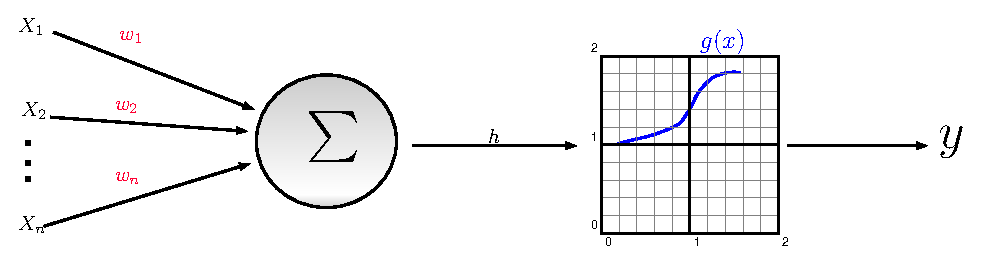
\includegraphics[scale=0.7]{Imagens/McCulloch.eps}
	}
	\caption{Modelo esquemático de um neurônio de McCulloch-Pitts. Onde $x_{1}, x_{2}, ..., x_{n}$ são os \textit{inputs}, $w_{1}, w_{2}, ..., w_{n}$ são os pesos, h é o treino, $g(x)$ é a função de ativação, e $y$ é o \textit{output}.}
	\label{Esquematico de McCulloch}
\end{figure}

Mais de $50$ tipos de redes neuronais artificiais tem sido criadas até o ano de $2014$ \citep{Saljooghi2014}.


\section{A Rede de Kohonen}

Neste trabalho, foi utilizada a rede de kohonen. Esta rede neuronal tem como importante característica ser uma rede com aprendizado não-supervisionado, portanto o espaço solução de saída da rede não é conhecido. 

A localização espacial de um neurônio da saída em um mapa topológico
corresponde a um domínio ou característica particular do dado retirado do espaço de entrada. E estas entradas são mapeadas de forma ordenada, a exemplo dos mapas cito-arqueturais do córtex cerebral.

Neste processo de identificação de padrões a redundância torna-se impreterível,
pois o neurônio da camada de saída que apresentar a maior resposta terá os seus
pesos ajustados. Além disso, o peso dos neurônios vizinhos também serão
ajustados em menor intensidade ao comparados com o neurônio vencedor.

Isto implica que os neurônios devem estar posicionados em um arranjo geométrico
adequado. Esta teoria é baseada na suposição de que as células nervosas
corticais estão organizadas anatomicamente em relação aos estímulos que recebem
dos sensores aos quais estão ligadas \citep{Artero2009}.

Este modelo exige a definição de vizinhança entre neurônios de forma geométrica. Alguns arranjos são comumente utilizados, como por exemplo, os arranjos triangulares, hexagonal, retangulares, etc.

No caso de arranjos retangulares, diferentes vizinhanças de um neurônio
$N_{i,j}$ podem ser configuradas em quartetos, diagonais e octetos. 

A Fig. \ref{hiperplano} ilustra o arranjo retangular e as vizinhanças, em quartetos, adotado neste trabalho. 

\begin{figure}[H]
	\centering
	\setlength{\fboxsep}{8pt}
	\setlength{\fboxrule}{0.1pt}
	\fbox{
		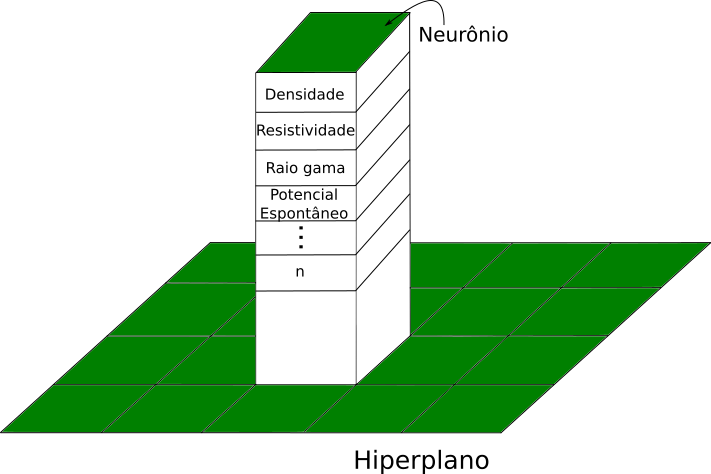
\includegraphics[scale=0.5]{Imagens/hiperplano.png}
	}
	\caption{Neurônio e suas vizinhanças}
	\label{hiperplano}
\end{figure}

O conceito de vizinhança representa uma competição pelo melhor aprendizado e o ajuste do vencedor e da sua vizinhança é um estímulo para que os neurônios ao redor do vencedor também melhorem.

Durante a etapa de treinamento é identificado o neurônio que tem os parâmetros de entrada mais parecidos com os valores dos pesos. Este procedimento é realizado via cálculo da distância euclidiana, Eq. \ref{euclidiana}, entre o parâmetro de entrada $x(t)$ e o peso $w_{i,j}$.

\begin{eqnarray}
d(t)= \sum^{n}_{i=1}[x(t)-w_{i,j}(t)]^{2}
\label{euclidiana}
\end{eqnarray}

A etapa de treinamento da rede se dá por um ajuste de pesos entre os neurônios através do cálculo do menor valor de $d(t)$ na iteração $t$, caracterizando assim o neurônio que passar por esse processo de \textit{vencedor}. Esse procedimento ajusta da mesma forma os pesos do neurônio da vizinhança dentro. Os pesos são ajustados co uma fração da diferença entre os \textit{inputs} $x_{i}$ e os pesos $w_{i}$, vide Eq.\ref{ajuste de pesos}.

\begin{equation}
w_{i,j}(t+1)=w_{i,j}(t)+n(t)[x(t)-w_{i,j}]
\label{ajuste de pesos}
\end{equation}

Através deste ajuste continuado de pesos os elementos do conjunto de entrada são reorganizados de tal foma que as classes próximas sejam posicionados umas perto das outras. Isso gera um mapa bi-dimensional denominado na literatura de \textit{mapa auto-organizável}. Este mapa é o análogo matemático mais fiel das áreas especializadas do córtex cerebral que são ilustradas pelo \textit{Homúnculo de Penfield}, \ref{homunculo}.

\section{Redes com aprendizado não-supervisionado}

Nesta categoria de RNA's são apenas inseridos os valores de \textit{input} da rede. Os \textit{output} são definidos pela própria rede que passa por um processo de treinamento não supervionado. As redes que são submetidas a este tipo de treinamento são mais indicadas para tarefas aonde são exigidos agrupamento de dados (\textit{clustering}). Neste processo uma classe deve ser atribuída aos registros da rede observando-se apenas o comportamento de seus atributos, no caso em particular deste trabalho tratam-se de propriedades geofísicas.

Uma rede com treinamento não supervisionado inspira-se no funcionamento do córtex cerebral. Neste modelo biológico, o organismo aprende a realizar alguma tarefa, por meio da identificação de padrões. Por exemplo, ao identificar uma música determinados padrões sonoros que compõe o conjunto harmonioso de notas precisam ser aprendidos antes de serem reconhecidos. Durante este processo, regiões específicas do cérebro vão sendo paulatinamente acionadas. Isto somente é possível, devido conexões específicas que são formadas entre os neurônios
presentes no córtex, Fig. \ref{homunculo}.

Os detalhes dos processos que regulam o córtex ainda não foram totalmente elucidados, contudo é seguro assumir que a primeira representação dos fenômenos de aprendizagem podem ser representados por uma superfície topológica ou mapa auto-organizado. 

\begin{figure}[H]
	\centering
	\setlength{\fboxsep}{8pt}
	\setlength{\fboxrule}{0.1pt}
	\fbox{
		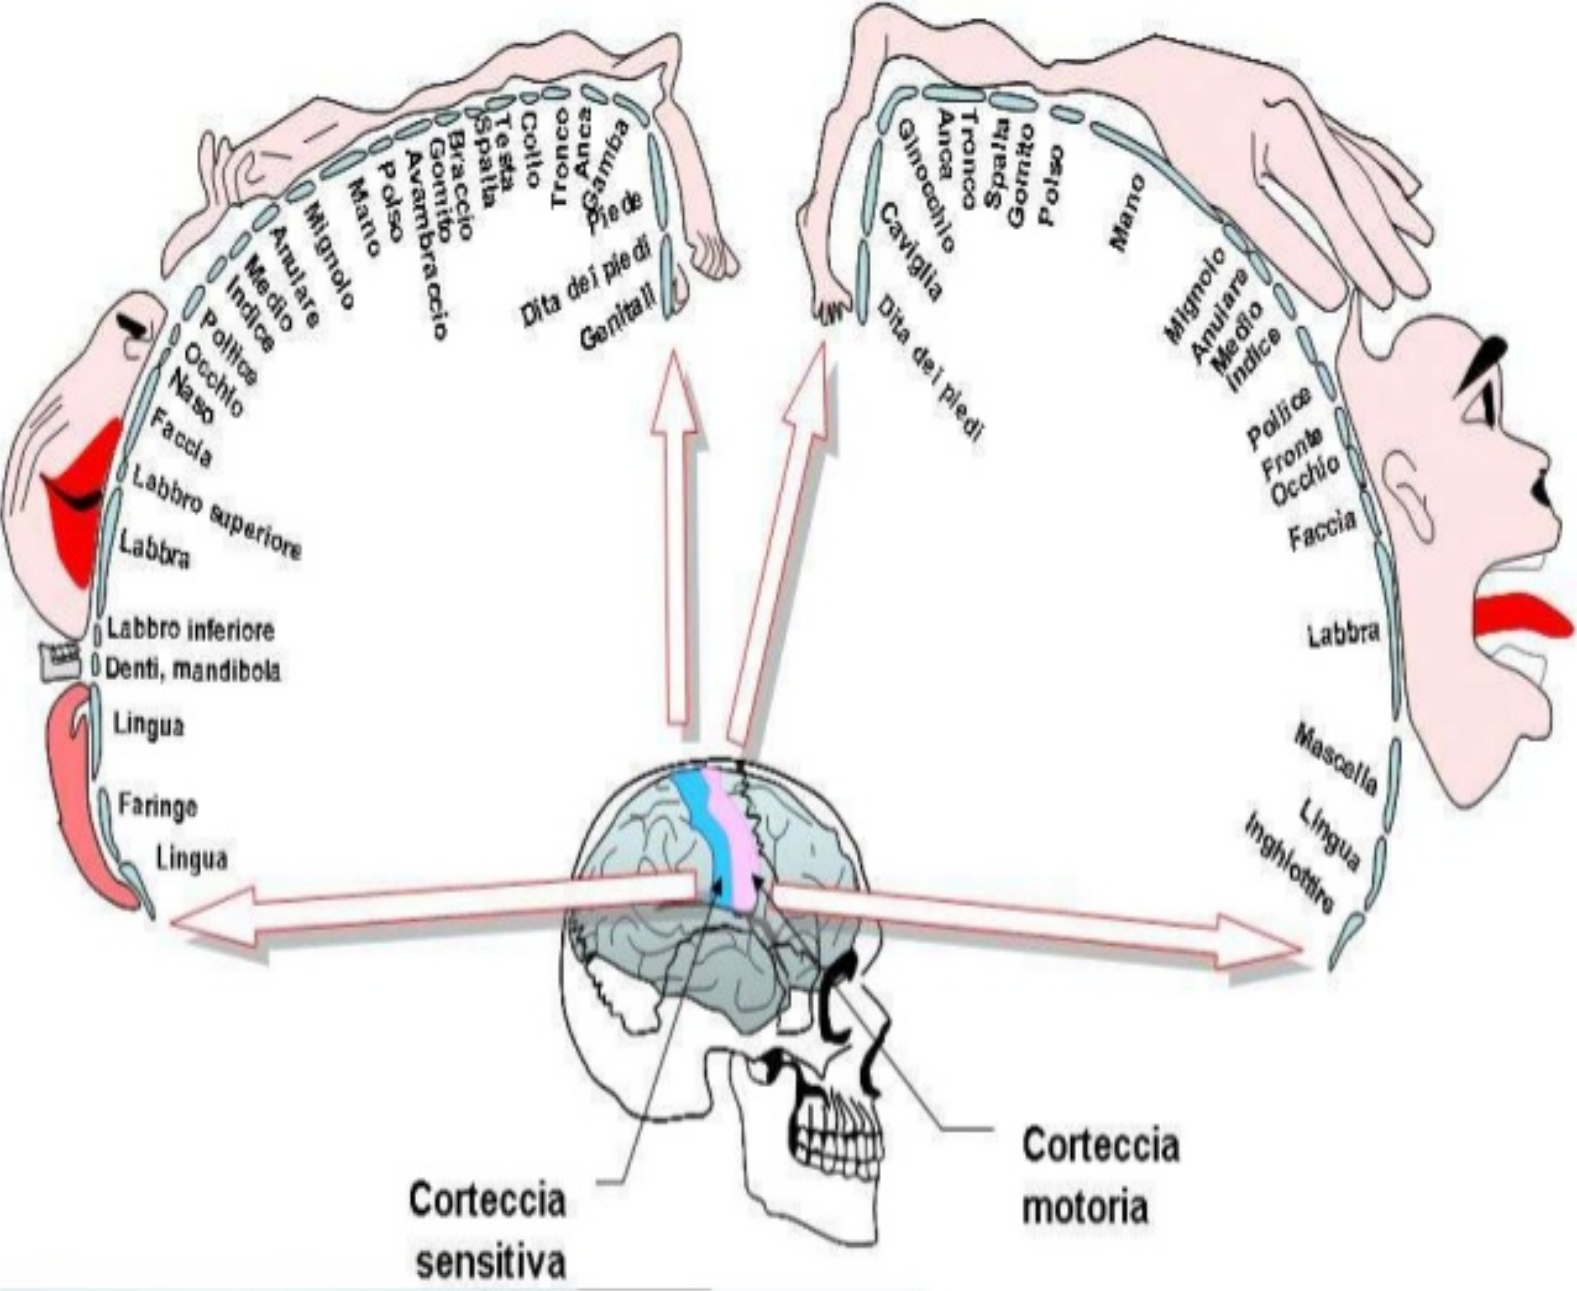
\includegraphics[scale=0.5]{Imagens/homunculo.png}
	}
	\caption{Homúnculo de Penfield.}
	\label{homunculo}
\end{figure}

Um cérebro que sofreu uma comossão grave perde a capacidade de acessar
determinadas zonas do homúnulo responsáveis por atividades específicas. Contudo
o cérebro tem a capacidade de destinar outras regiões para o controle destas
ações que foram previamente perdidas.

Além de casos graves como um acidente o cérebro também perde a capacidade de
aprendizado com o tempo. Em humanos, a capacidade de aprendizado vai da pequena
infância até a puberdade. Após este período, o cérebro passar a reter o que fora
aprendido. Sendo assim o aprendizado é uma função que depende, entre outras
coisas, do tempo.

  \chapter{Justificativa para escolha do tema}

Para ilustrar a completa ades\~ao ao estilo de cita{\c c}\~oes e listagem de
refer\^encias bibliogr\'aficas, a Tabela~\ref{tab:citation} apresenta cita{\c
c}\~oes de alguns dos trabalhos, utilizando o estilo alfabético (default). Para
utilização do estilo numérico, deve-se utilizar a opção number da classe ON, ou seja,
basta usar \verb|\documentclass[dsc, numbers]{on}|.

\begin{table}[h]
\caption[Exemplos de tabela (texto do índice)]{Exemplos de tabela mostrando os comandos para
  cita{\c c}\~oes utilizando o comando padr\~ao \texttt{\textbackslash citep} do \LaTeX\ e
  o comando \texttt{\textbackslash citet},
  fornecido pelo pacote \texttt{natbib}.}
\label{tab:citation}
\centering
{\footnotesize
\begin{tabular}{|c|c|c|}
  \hline
  Tipo da Publica{\c c}\~ao & \verb|\citep| & \verb|\citet|\\
  \hline
  Livro & \citep{book-example} & \citet{book-example}\\
  Artigo & \citep{article-example} & \citet{article-example}\\
  Relat\'orio & \citep{techreport-example} & \citet{techreport-example}\\
  Relat\'orio & \citep{techreport-exampleIn} & \citet{techreport-exampleIn}\\
  Anais de Congresso & \citep{inproceedings-example} &
    \citet{inproceedings-example}\\
  S\'eries & \citep{incollection-example} & \citet{incollection-example}\\
  Em Livro & \citep{inbook-example} & \citet{inbook-example}\\
  Disserta{\c c}\~ao de mestrado & \citep{mastersthesis-example} &
    \citet{mastersthesis-example}\\
  Tese de doutorado & \citep{phdthesis-example} & \citet{phdthesis-example}\\
  \hline
\end{tabular}}
\end{table}

%\section{seção 1}


  \chapter{Objetivos geral e espec\'{i}ficos}

  \chapter{Metodologia}

Um exemplo de utilização de equações matemáticas é apresentado abaixo na Equação~\ref{eq:nome1}:
\begin{equation}
\label{eq:nome1}E=mc^2
\end{equation}

Para um conjunto de equações, como as Equações~\ref{eq:nome2}-\ref{eq:nome3}:
\begin{eqnarray}
\label{eq:nome2} & & \;\;\;\;\; \rho \partial_t v_i
 - \partial_j \tau_{ij} = f_i\\
\label{eq:nome3} & &
\partial_t \tau_{ij}-c_{ijkl}\partial_l v_{k}=-\partial_tg_{ij},
\end{eqnarray}


Um exemplo de utilização de figuras no \LaTeX é apresentado a seguir: na
Figura~\ref{fig:caption1} é mostrado uma figura-exemplo contendo um snapshot
de uma propagação de ondas elásticas em um meio anisotrópico.
\begin{figure}[hbt]
\centering 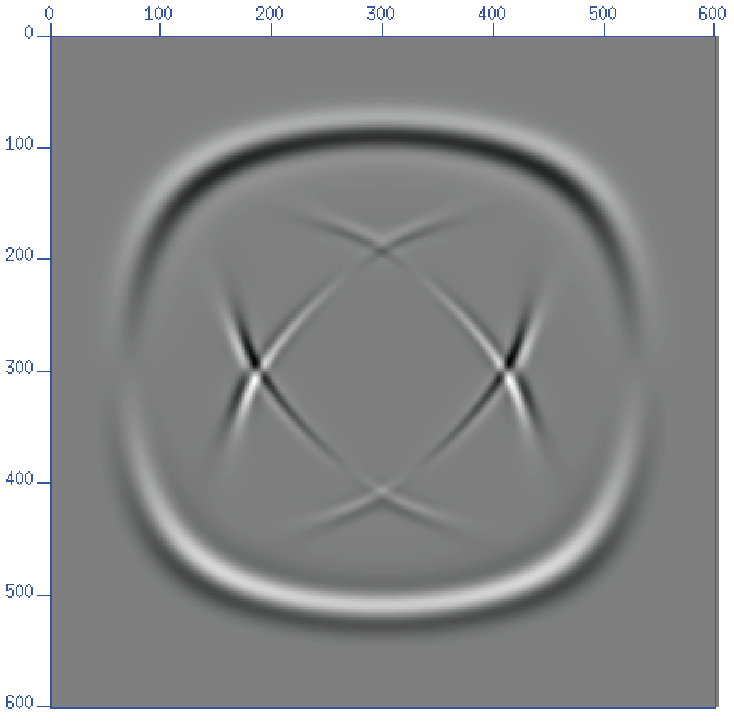
\includegraphics[width=6.5cm,height=6.5cm]{Figs/snap}
\caption[Exemplo de figura simples (texto do índice).]{Exemplo de figura simples:
modelagem elástica de um meio anisotrópico.}
\label{fig:caption1}
\end{figure}

Exemplo de utilização de figuras múltiplas é apresentado na Figura~\ref{fig:cc}
abaixo. Podemos referenciar cada uma das figuras, por exemplo a Figura~\ref{fig:cc_nr} ou
a Figura~\ref{fig:cc_cerjan}.
\begin{figure}[hbt]
\centering \subfigure[Condição de contorno não reflexiva
(CCNR).]{\label{fig:cc_nr}
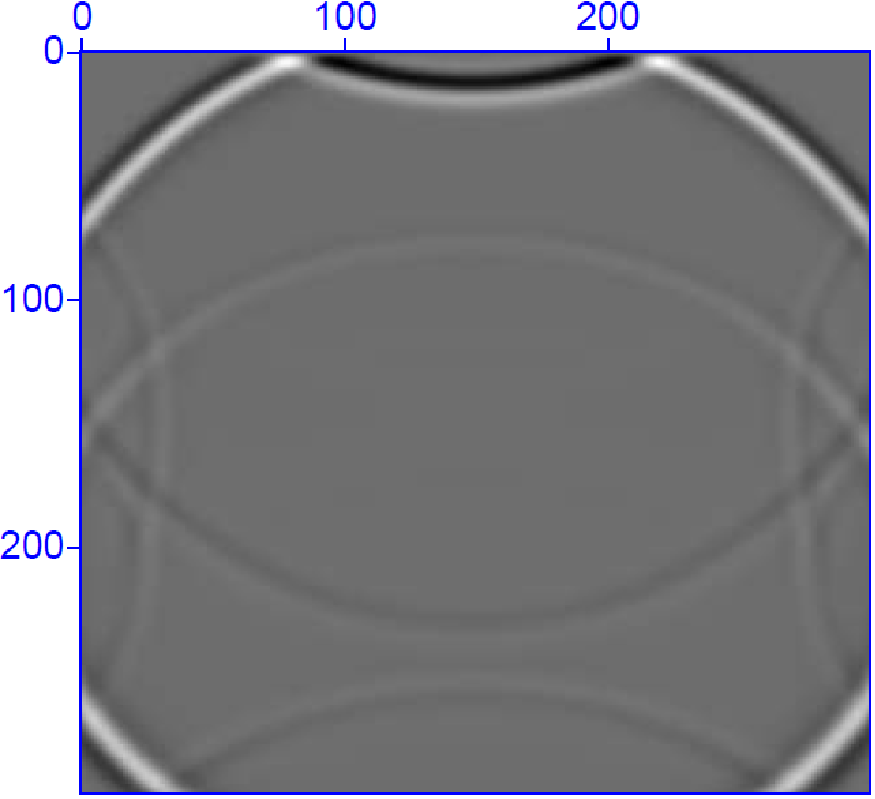
\includegraphics[width=6.5cm,height=6.5cm]
{Figs/cc_nr}} \qquad \subfigure[Camadas de amortecimento +
CCNR.]{\label{fig:cc_cerjan}
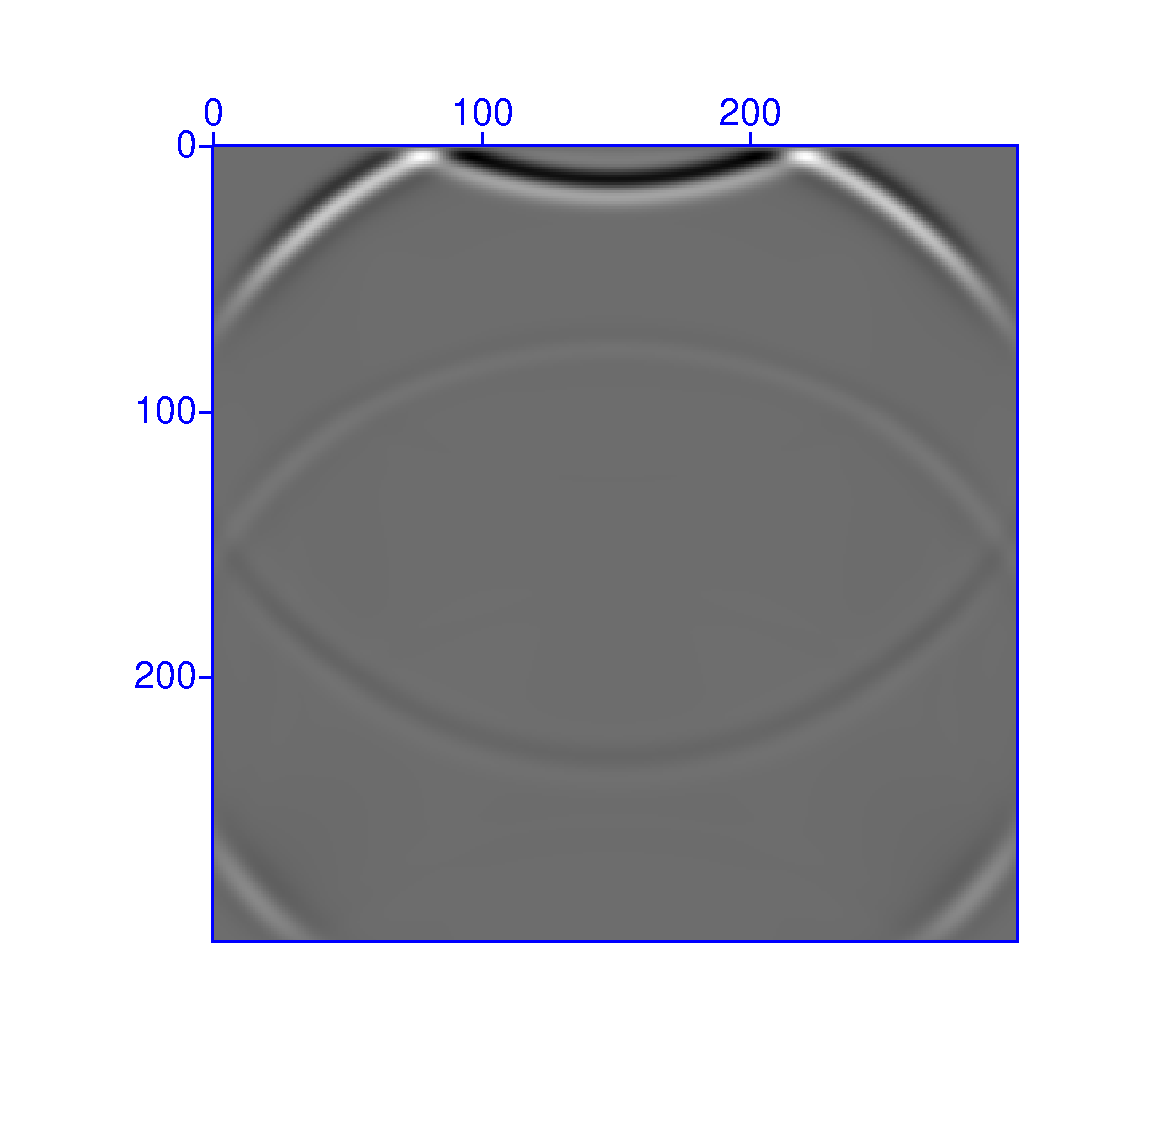
\includegraphics[width=6.5cm,height=6.5cm]{Figs/cerjan}}
\caption[Exemplo de múltiplas figuras (texto do índice).]{Exemplo de múltiplas
figuras: modelagem
acústica mostrando efeito da aplicação da CCNR e camadas de amortecimento
aplicadas nas bordas (menos na superfície). Aplica-se em (a) as CCNR de
Reynolds e em (b) as camadas de amortecimento mais CCNR de Reynolds.}
\label{fig:cc}
\end{figure}

Repare para que o exemplo acima funcione corretamente, é necessário a utilização do pacote``\verb|\usepackage{subfigure}|'', declarado no preambulo do documento principal. Para tal, este pacete deve estar instalado no LaTex utilizado para processar o documento. Indicamos a utilização do MikTex (gratuito) mais atual com editor WinEdt (pago).
  \chapter{Resultados e Discussões}

A Fig. \ref{clusterT1} apresenta à análise de agrupamentos das propriedades físicas analisadas por classes de rochas para o poço T$1$. Foi utilizado para tal foi adotado um padrão de cores para cada tipo litológico. 

\begin{figure}[H]
	\centering
	\setlength{\fboxsep}{8pt}
	\setlength{\fboxrule}{0.1pt}
	\fbox{
		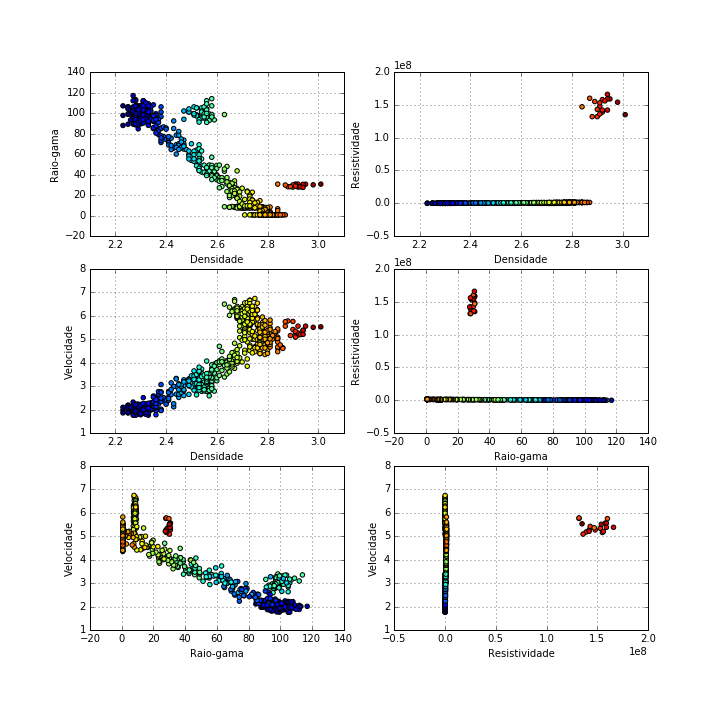
\includegraphics[scale=0.5]{Imagens/cluterpocoT1.png}
	}
	\caption{Agrupamento de dados do poço T1.}
	\label{clusterT1}
\end{figure} 

Em vermelho escuro, se encontra o diabásio, a gradação de cores entre o vermelho claro e o amarelo, se encontra o embasamento, a gradação de cores entre o laranja e o verde claro encontra-se a dolomita, verde claro se encontra o folhelho $2$, a gradação de azul para azul escuro encontra-se o conglomerado, e a gradação que vai do amarelo ao azul são as subclasses de mistura de conglomerado com embasamento de $20\%$, $40\%$, $60\%$ e $80\%$, respectivamente.

É perceptível o notável contraste de variação de resistividade entre a rocha de origem ígnea, em contraste com as propriedades físicas das demais rochas de origem sedimentar e metamórfica. O agrupamento das rochas sedimentares formam um conjunto quase linear próximo a zero.

A Fig. \ref{clusterC1} apresenta à variação das propriedades físicas analisadas por agrupamento de classes de rochas para o poço C$1$.

\begin{figure}[H]
	\centering
	\setlength{\fboxsep}{8pt}
	\setlength{\fboxrule}{0.1pt}
	\fbox{
		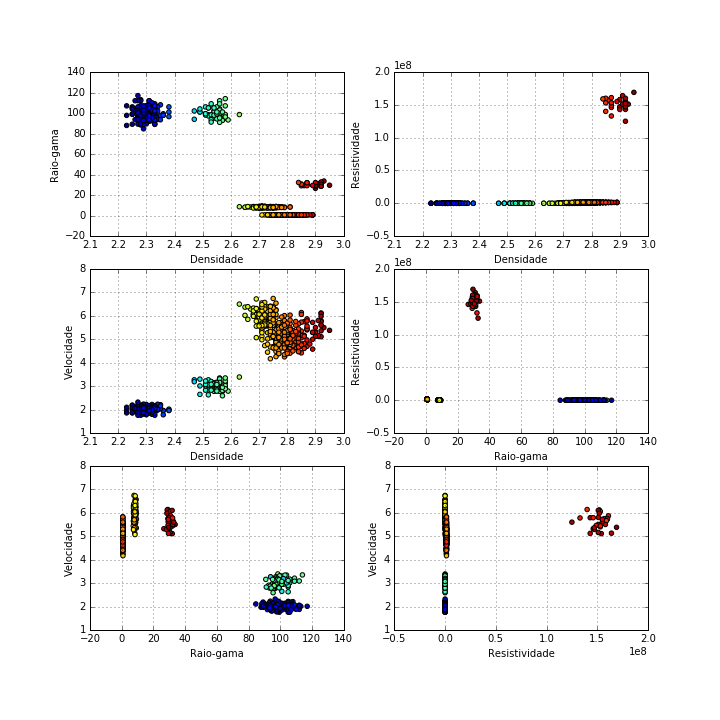
\includegraphics[scale=0.5]{Imagens/cluterpocoC1.png}
	}
	\caption{Agrupamento de dados do poço C1.}
	\label{clusterC1}
\end{figure} 

Neste caso, o agrupamento das classes de rochas é mais evidente, no gráfico de raio-gama por densidade, que evidencia os $5$ litotipos distintamente. E, da mesma maneira, o gráfico de velocidade por densidade.


A Fig. \ref{clusterC2} apresenta à variação das propriedades físicas analisadas por agrupamento de classes de rochas para o poço C$2$. Em destaque, de vermelho, o litotipo diabásio. 

\begin{figure}[H]
	\centering
	\setlength{\fboxsep}{8pt}
	\setlength{\fboxrule}{0.1pt}
	\fbox{
		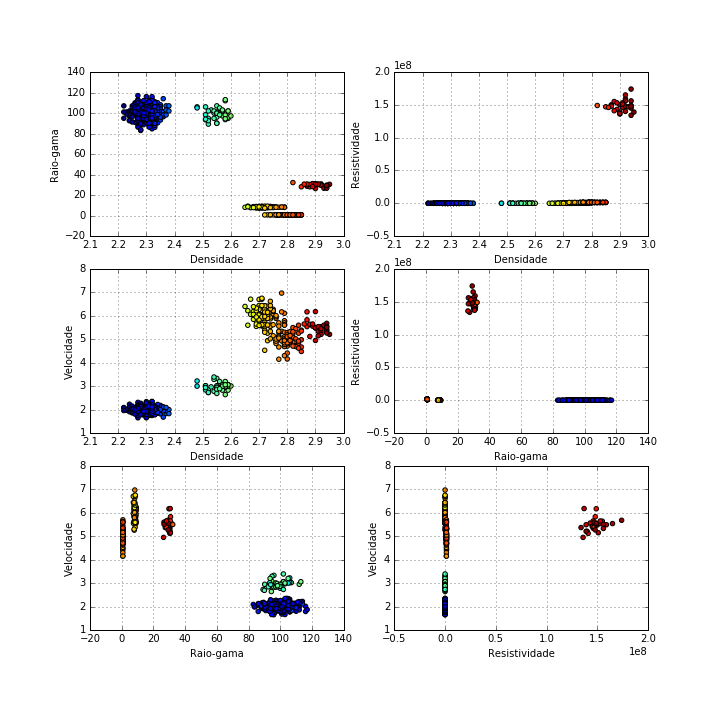
\includegraphics[scale=0.5]{Imagens/cluterpocoC2.png}
	}
	\caption{Agrupamento de dados do poço C2.}
	\label{clusterC2}
\end{figure} 

Na mesma forma, o agrupamento das classes de rochas é mais evidente, no gráfico de raio-gama por densidade, que evidencia os $5$ litotipos distintamente. E, da mesma maneira, o gráfico de velocidade por densidade.

\section{Treinamento}

A etapa de treinamento consiste em um ajuste de pesos dos neurônios da rede. Nesta fase, é identificado o neurônio que tem os valores dos pesos mais parecidos com os parâmetros de entrada da rede.  Por conseguinte, os diversos mapas são obtidos através dos sucessivos ciclos de treinamento ao longo do tempo. A Fig. \ref{SOM}(a), representa a organização da rede com apenas um ciclo de treinamento. Nesta imagem, a rede ainda não é capaz de identificar nenhuma litologia. Ao se aumentar o número de ciclos é perceptível que o ajuste dos pesos cria um conjunto de neurônios vencedores capazes de identificar as classes litológicas. Na quinta iteração, Fig. \ref{SOM}(b), as classes folhelho 2 e dolomita, por exemplo (cores mais azuis) ocupam a maior área do mapa. Já na milésima iteração, Fig. \ref{SOM}(d), a área azul é reduzida dando lugar as cores amarela e verde, que representam as subclasses de conglomerado e embasamento.

\begin{figure}[H]
\centering
\subfigure[ref1][Iteração 1]{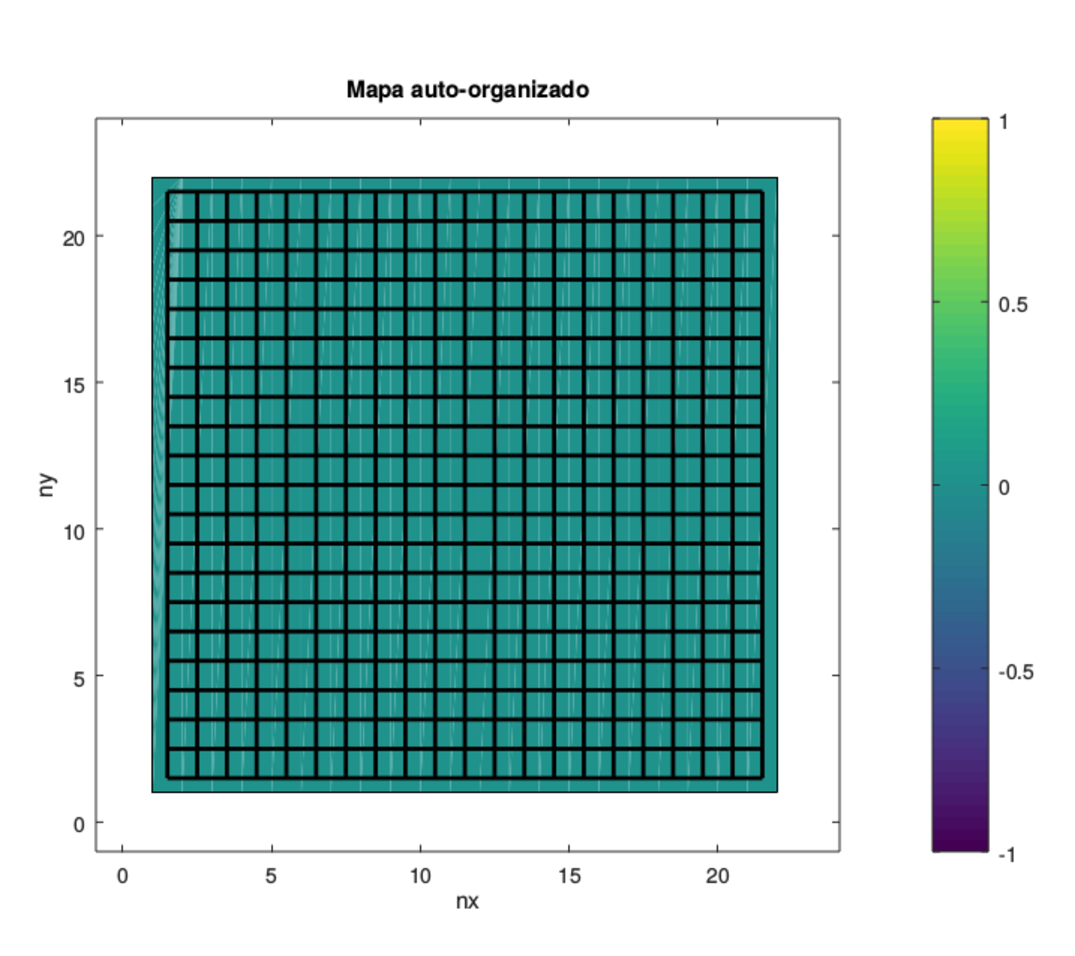
\includegraphics[width=7.0cm]{Imagens/SOM1_2d.pdf}}
\qquad
\subfigure[ref2][Iteração 5]{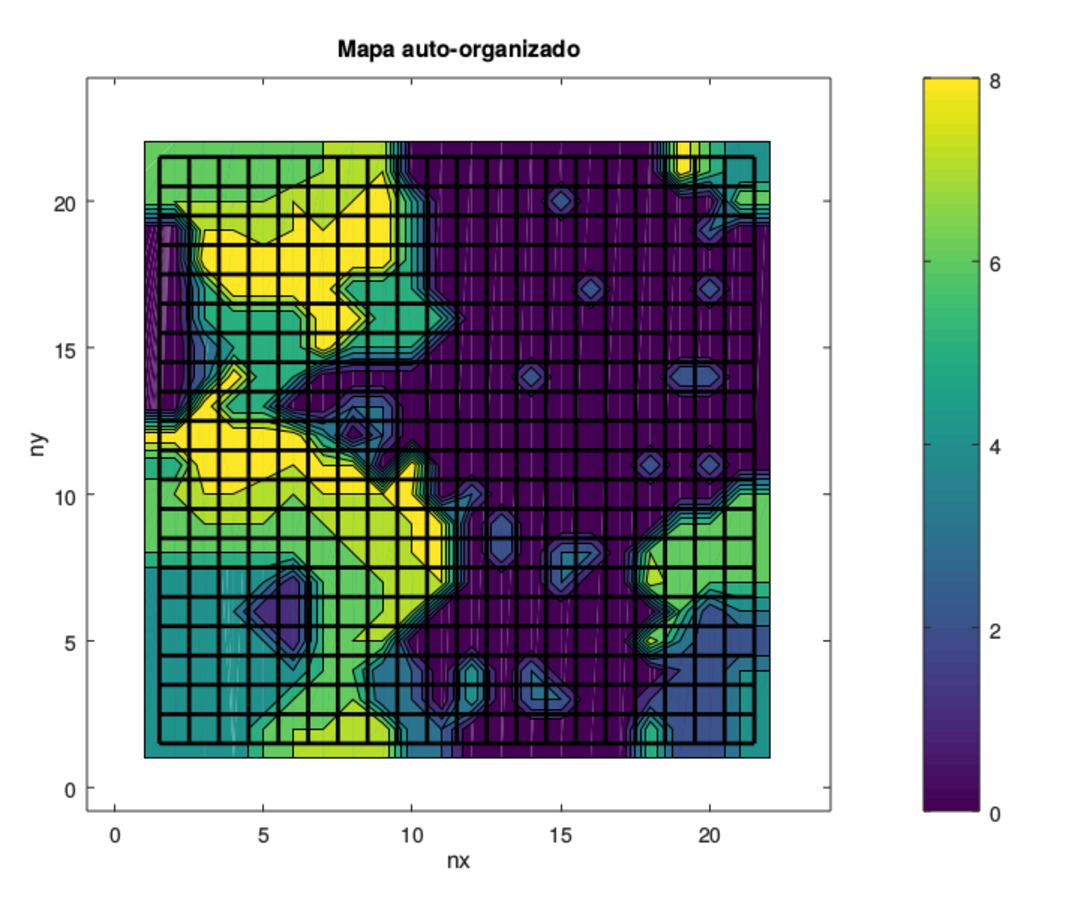
\includegraphics[width=7.0cm]{Imagens/SOM5_2d.pdf}}
\qquad
\subfigure[ref3][Iteração 100]{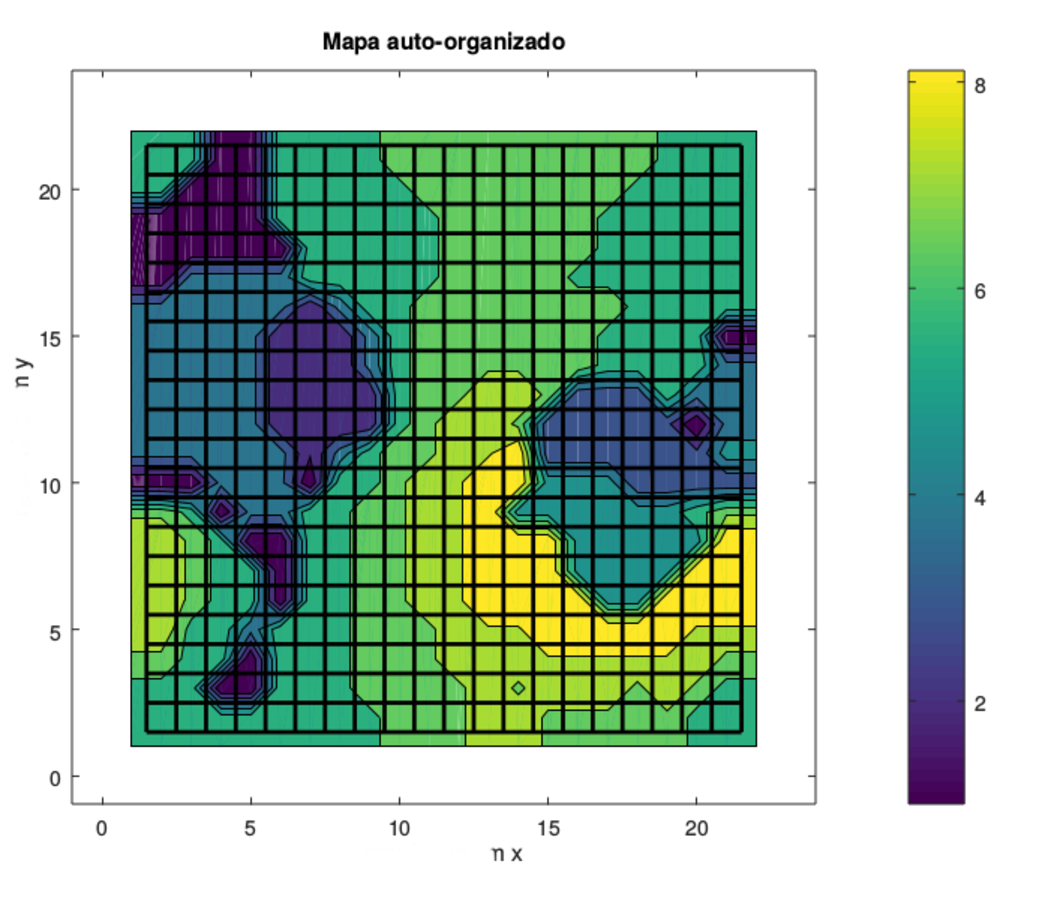
\includegraphics[width=7.0cm]{Imagens/SOM100_2d.pdf}}
\qquad
\subfigure[ref4][Iteração 1000]{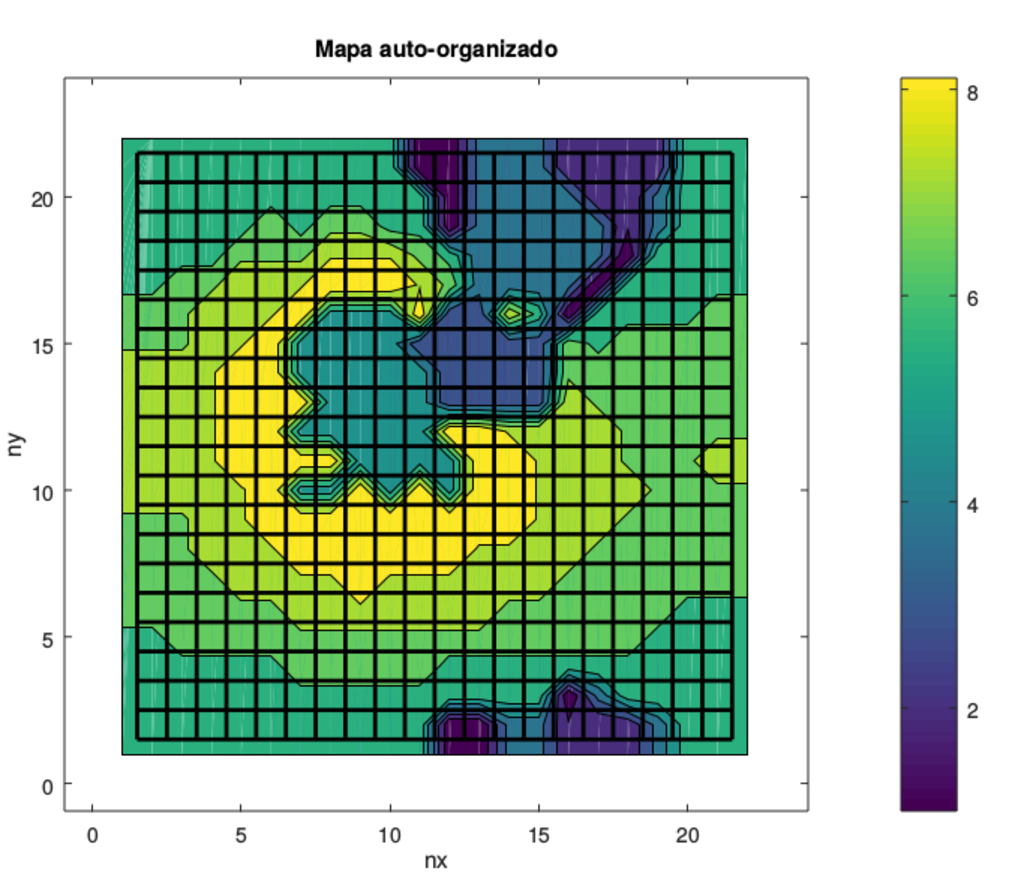
\includegraphics[width=7.0cm]{Imagens/SOM1000_2d.pdf}}
\qquad
\caption{Mapas auto-organizáveis e sua evolução temporal.}
\label{SOM}
\end{figure}

Os mapas da Fig. \ref{SOM} apresentam as zonas do hiperplano especializadas em identificar as classes de rochas. O código numérico $1$ representa folhelho, $2$ dolomita, $3$ diabásio, $4$ conglomerado, $5$ embasamento, $6$ mistura conglomerado/embasamento $80\%$, $7$ mistura conglomerado/embasamento $60\%$, $8$ mistura conglomerado/embasamento $40\%$ e $9$ mistura conglomerado/embasamento $20\%$ . A Tab. \ref{codigos} faz um paralelo entre o código numérico utilizado com \textit{output} da rede e as litologias do modelo.

\begin{table}[H]
	\centering
	\begin{tabular}{c|c}
		
		Litologia                    & Código numérico \\ % Note a separação de col. e a quebra de linhas
		\hline                                                             % para uma linha horizontal
		Folhelho 2                 &  1\\
		Dolomita  		            &  2 \\
		Diabásio    	            &  3 \\
		Conglomerado          &  4 \\
		Conglomerado 80\% &  5  \\
		Conglomerado 60\%&  6 \\
		Conglomerado 40\%&  7\\
		Conglomerado 20\%&  8 \\
		Embasamento          &  9 \\
	 % não é preciso quebrar a última linha
		
	\end{tabular}
	\label{codigos}
	\caption{Tabela de referência para conversão do padrão numérico em litologia.}
\end{table}

A Fig. \ref{convergencia} apresenta o teste de convergência da rede neuronal.

\begin{figure}[H]
	\centering
	\setlength{\fboxsep}{8pt}
	\setlength{\fboxrule}{0.1pt}
	\fbox{
		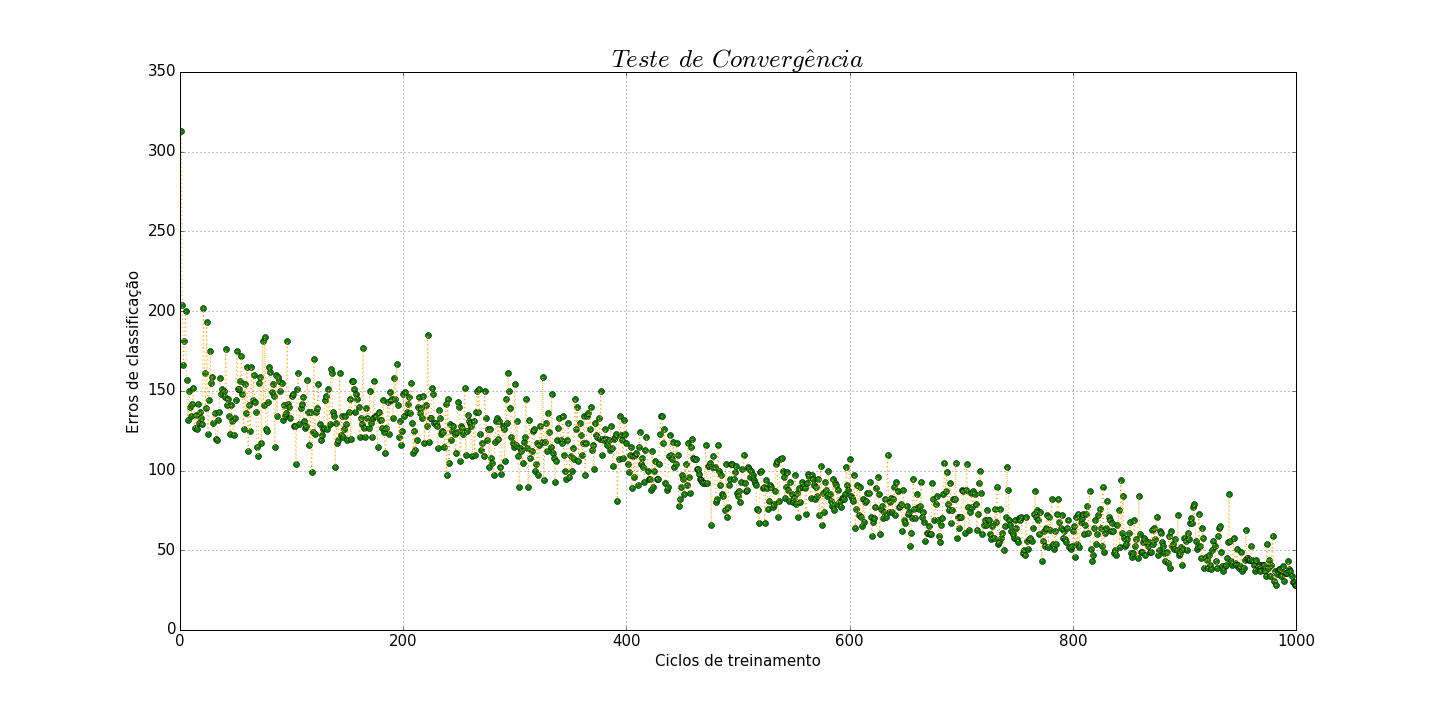
\includegraphics[scale=0.3]{Imagens/conv070917.png}
	}
	\caption{Teste de convergência da rede.}
	\label{convergencia}
\end{figure} 

O teste de convergência é realizado durante a fase de treinamento e mostra que a rede se encontra estabilizada em  $1000$ ciclos de treinamento com $28$ erros de classificação, ou seja, um erro de $4\%$. Isto significa ser inócuo aumentar a iteração afim de diminuir o erro. 



\section{Identificação}

A seguir são apresentados os resultados da etapa de classificação da rede foram acrescentados os resultados dos classificadores euclideanos e de Mahalanobis. Nesta fase, dois poços foram utilizados chamados de poços C$1$ e C$2$. O primeiro destes localizado a SW do perfil, Fig. \ref{modelo}, possui $7$km de profundidade. A saída da rede, para o poço C$1$ está localizada ao lado direito da Fig. \ref{Class C1}. Ao lado esquerdo é apresentada o poço original. Abaixo é mostrado uma breve estatística deste processo de identificação da rede. Ao lado esquerdo do poço identificado pela rede estão os resultados obtidos pelos classificadores euclideano e de Mahalanobis. 


\begin{figure}[H]
	\centering
	\setlength{\fboxsep}{8pt}
	\setlength{\fboxrule}{0.1pt}
	\fbox{
		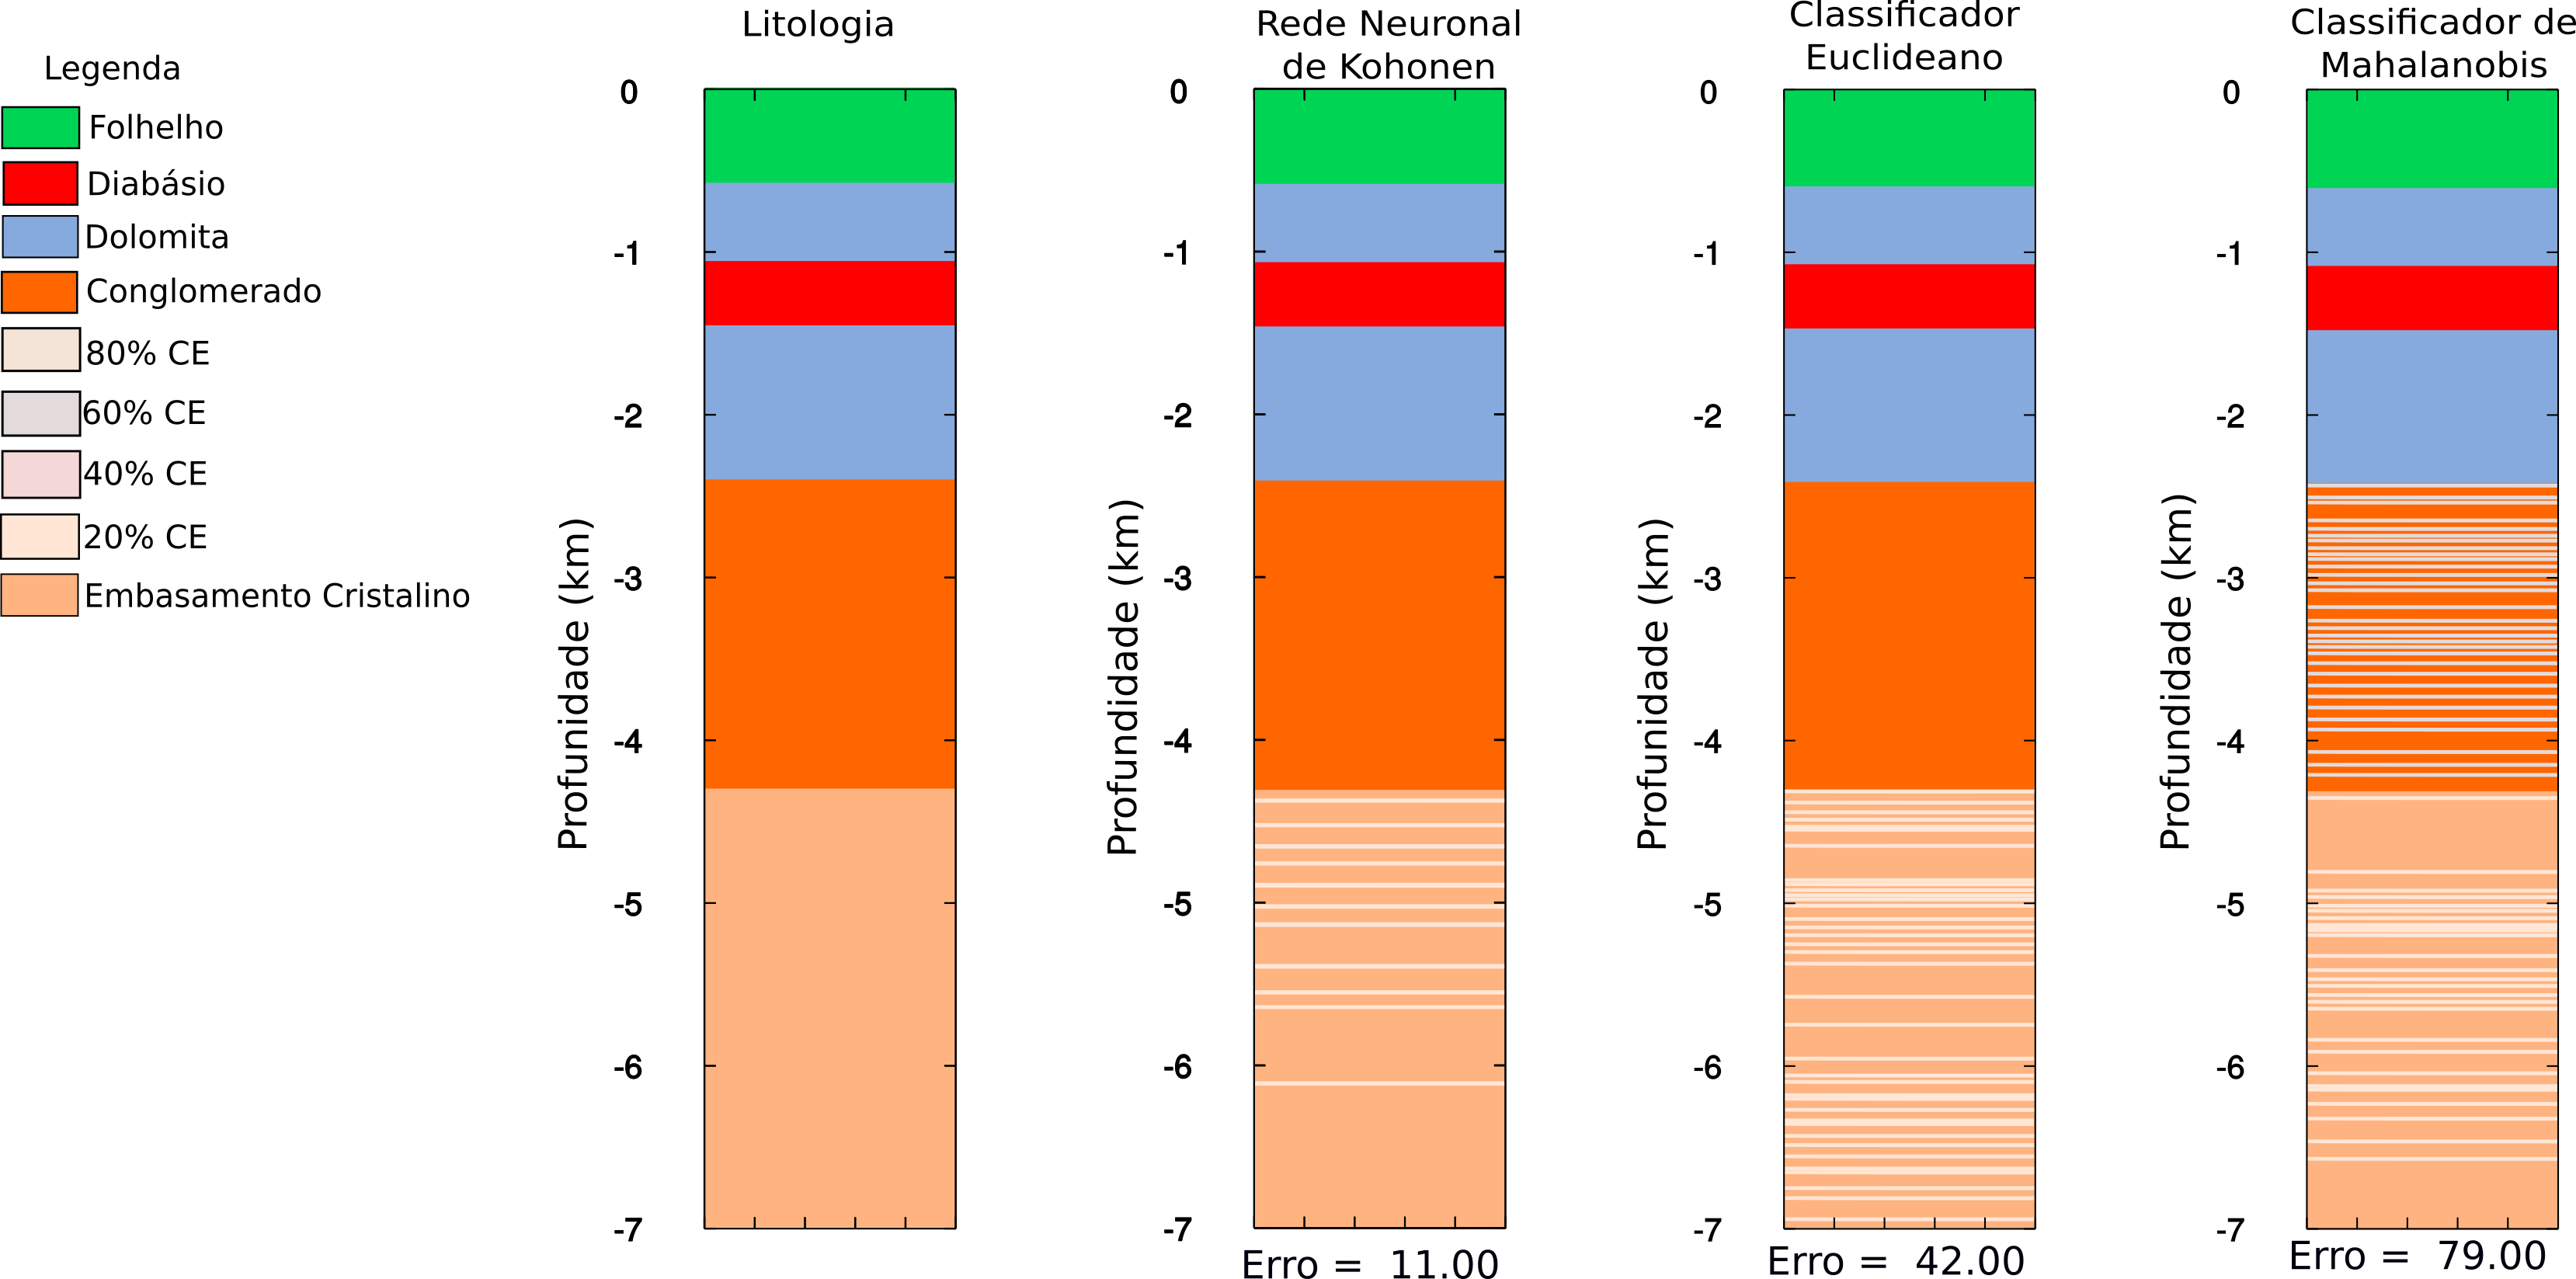
\includegraphics[scale=0.5]{Imagens/IDC1020118.png}
	}
	\caption{Dado de saída da rede para o poço de classificação C1.}
	\label{Class C1}
\end{figure} 


O processo de identificação foi repetido, contudo, desta vez, para o caso do ao poço C$2$. Este localiza-se mais a NE do perfil, Fig. \ref{modelo}, no topo de um alto estrutural com igual profundidade de $7$ km. A saída da rede, para o poço C$2$ está localizada ao lado direito da Fig. \ref{Class C2}. Ao lado esquerdo é apresentada o poço original. Abaixo é mostrado uma breve estatística do processo de identificação.  Ao lado esquerdo do poço identificado pela rede estão os resultados obtidos pelos classificadores euclideano e de Mahalanobis.  


\begin{figure}[H]
	\centering
	\setlength{\fboxsep}{8pt}
	\setlength{\fboxrule}{0.1pt}
	\fbox{
		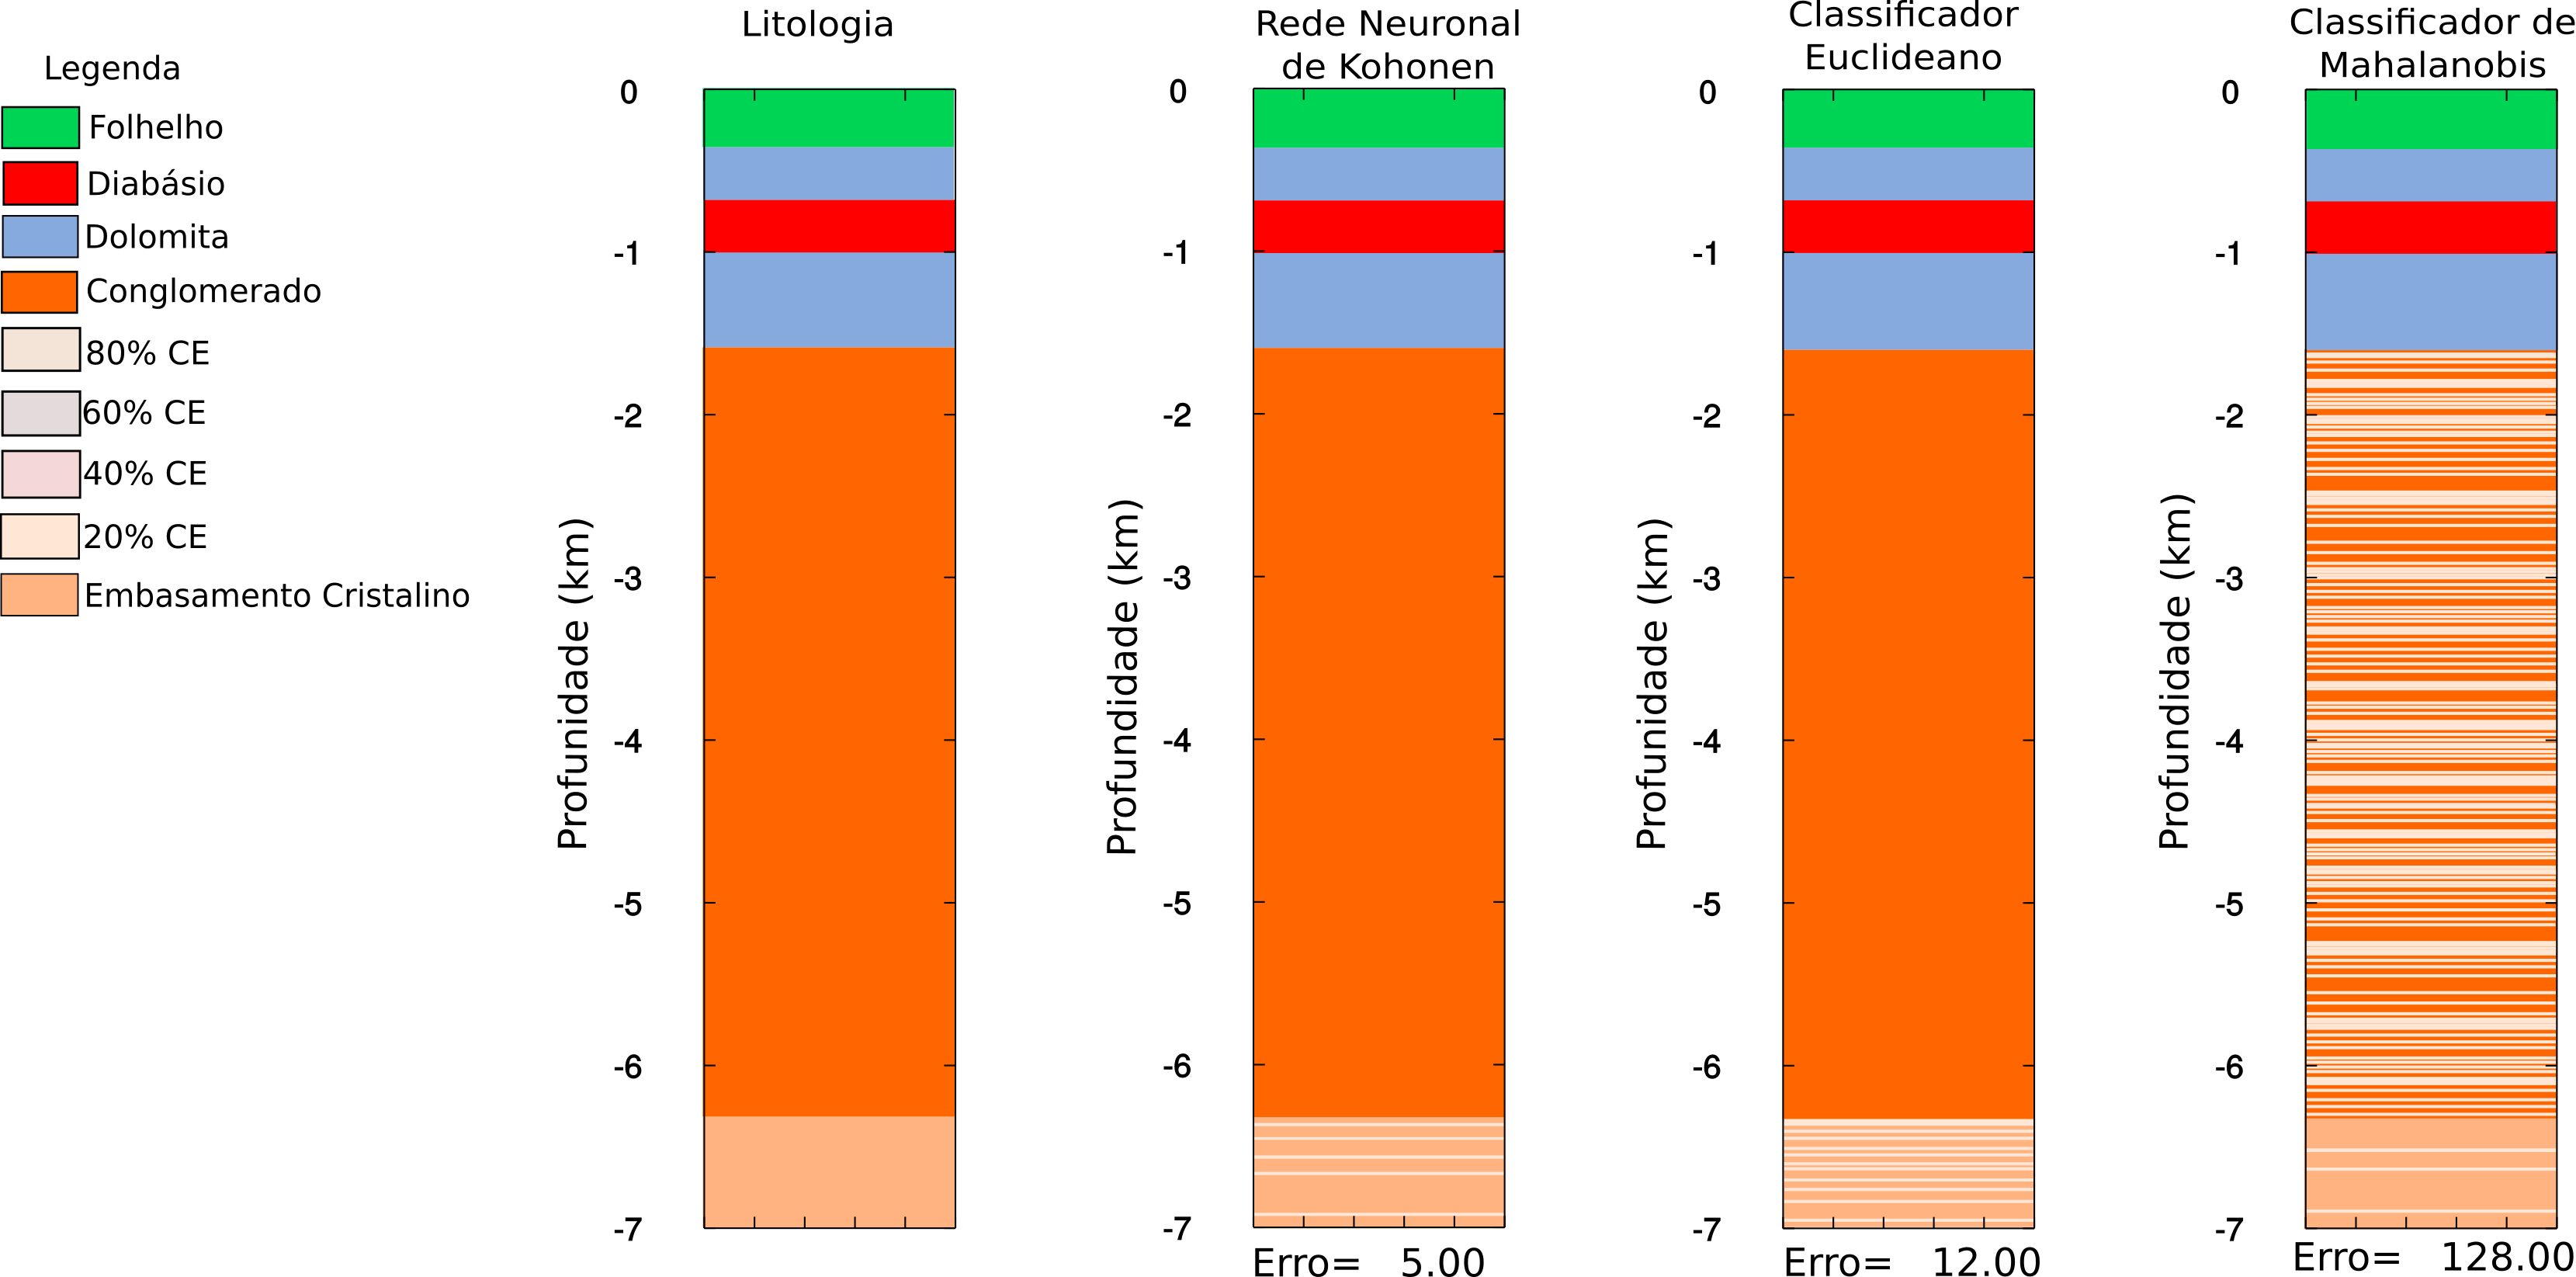
\includegraphics[scale=0.5]{Imagens/IDC2020118.png}
	}
	\caption{Dado de saída da rede para o poço de classificação C2.}
	\label{Class C2}
\end{figure} 


Em ambos os casos de identificação, o número de neurônios vitoriosos igualou-se ao total de neurônios da rede, Tab. \ref{Estatistica da rede}. Isto indica o máximo de aproveitamento durante os processos, com um tempo de máquina atingindo $25$ segundos. 


\begin{table}[H]
	\centering
	\caption{}
	\label{Estatistica da rede}
	\begin{tabular}{@{}lcc@{}}
		\toprule
		\multicolumn{3}{c}{Estatística da Rede}         \\ \midrule
		Dados                       & Poço C1 & Poço C2 \\
		Dados de treinamento        & 697     & 697     \\
		Dados a serem classificados & 699     & 698     \\
		Neurônios da Rede           & 400     & 400     \\
		Neurônios vitoriosos        & 400     & 400     \\
		Neurônios sem uso           & 0       & 0       \\
		Erro                        & 11      & 5       \\ \bottomrule
	\end{tabular}
\end{table} 


 Os classificadores apresentaram dois comportamentos distintos. No poço C$1$, o classificador de Euclides apresentou $42$ erros confundindo rochas do embasamento com rochas com $20\%$ de conglomerado e embasamento. No poço C$2$, o classificador de Euclides apresentou um maior número de erros $12$ associados ao embasamento cristalino classificando alguns pontos como conglomerado com $20\%$ de conglomerado e embasamento. 

Em contra-partida, o classificador de Mahalanobis apresentou $79$ erros, no total do poço C$1$ trocando as rochas do embasamento e conglomerado por dois tipos específicos de rocha: as rochas do $20\%$ e $60\%$ CE. E apresentou $128$ erros bem distribuídos ao longo das rochas do embasamento e conglomerado, no poço C$2$ confundindo-as com rochas de $60\%$ e $20\%$ de conglomerado com embasamento. 






  \chapter{Conclusões}

O teste de convergência da rede, Fig \ref{convergencia}, realizado durante a etapa de treinamento, indicou que o número de erros não iria diminuir após o milésimo ciclo de treinamento. Sendo o resultado, Fig. \ref{SOM}, deste teste usado como parâmetro para o número de repetições realizadas para os casos de identificação da rede. 

Os diagramas de velocidades por densidade e o de velocidade por raio-gama, Fig. \ref{clusterT1}, Fig. \ref{clusterC1} e Fig. \ref{clusterC2}, apresentaram os agrupamentos mais bem separados. Portanto estas propriedades físicas (densidade, velocidade e raio-gama) tem uma importância relativa maior ,na classificação das litologias dos poços C$1$ e C$2$. 

A saída da rede aponta que o maior caso de erros ocorreram em uma única classe de rocha, a do embasamento. Esses erros fizeram com que conglomerados fossem classificados como rochas do embasamento, nos dois casos dos poços de classificação, o poço C$1$ e o poço C$2$.  Uma das razões pode ser o fato das misturas de conglomerado e embasamento serem finas demais para a rede conseguir realizar uma identificação de padrão. Ou pelo fato dos conjuntos de propriedades físicas da mistura de $20\%$ se aproximar das propriedades físicas que representam o litotipo embasamento. 

O menor número de erros relativos encontrados, no poço C$2$, Fig. \ref{Class C2}, deve-se a escolha da alocação do furo, no perfil. O poço C$2$ localiza-se em um baixo estrutural, atingindo menos de $1$km do embasamento. Entretanto, o poço C$1$, Fig. \ref{Class C1}, encontra-se em um alto estrutural, divergindo do poço C$2$ e produzindo, consequentemente, os maiores erros relativos encontrados.    

O classificador de Euclides apresentou mais erros do que a rede neuronal de Kohonen com $42$ erros para o poço C$1$ e $12$ erros para o poço C$2$. E o classificador de Mahalanobis apresentou o resultado de identificação de poços com os maiores erros $79$ e $128$ respectivamente para os poços C$1$ e C$2$. 

Tal desempenho dos classificadores se deu por conta da existência de uma falha normal aonde foi escolhida a alocação do furo, Fig. \ref{modelo}. Nesta situação simulada há uma mistura entre os clusters em todos os espaços bi-dimensionais de propriedades analisadas tanto para o conglomerado quanto para o embasamento cristalino, Fig. \ref{clusterT1}. Portanto a definição dos centroides dos agrupamentos de propriedades ficam longe das distribuições ideais preditas no teste analítico do capítulo \ref{introducao}, na seção \ref{teste}.  



  \backmatter

  % estilo de citações por ordem alfabética (defaut da classe ONTeX)
  \bibliographystyle{on-plain}
  \bibliography{references}

  \appendix
  % A linha "\include" abaixo inclui um capítulo de apêndice.
  % Edite o arquivo "appenA.tex" de acordo com as suas necessidades.
  % É possível incluir outros capítulos de apêndice. Para tanto,
  % crie outros arquivos "appenX.tex", de acordo com as suas necessidades,
  % e inclua-os no documento utilizando "\include{appenX}".
  \chapter{Algumas Demonstrações}

Aqui devem entrar demonstrações mais longas, revisões de conceitos mais básicos
ou qualquer detalhe pertinente que não seja adequado para o corpo da
dissertação/tese.


\end{document} 